\documentclass[11pt, a4paper]{article}
\usepackage{graphicx}				
\usepackage{amssymb}
\usepackage{algorithm}
\usepackage{enumerate}
\usepackage[noend]{algpseudocode}
\usepackage{Sweave}
\usepackage{amsmath}
\usepackage{amsthm}
\usepackage{mathrsfs}
\usepackage{cite}

\makeatletter
\def\BState{\State\hskip-\ALG@thistlm}
\makeatother
\theoremstyle{plain}
\newtheorem{thm}{Theorem}[section] % reset theorem numbering for each chapter
\theoremstyle{definition}
\newtheorem{defn}[thm]{Definition} % definition numbers are dependent on theorem numbers
\newtheorem{exmp}[thm]{Example} % same for example numbers
\newtheorem{lem}[thm]{Lemma}
\newcommand{\R}{\mathbb{R}}
\newcommand{\supp}{\mbox{supp}~} 
\newcommand{\pr}{\mathrm{Pr}}

\title{Sampling from High Dimensional Distributions}
\author{Bill DeRose \\ Advisor: Gabe Chandler}
\begin{document}
\input{thesis_draft_2-concordance}
\input{thesis_draft_2-concordance}
\maketitle
\tableofcontents
\part{Introduction}
\section{Introduction}
The  difficulties we face in computational statistics are a consequence of modern technology.
%It is a consequence of modern technology that we face computational difficulties in the field of statistics. 
We should be so lucky to face the problem of designing algorithms to generate truly random numbers. And yet, we delude ourselves into believing there is randomness where there is none.

\begin{figure}[!htbp]
   \centering
   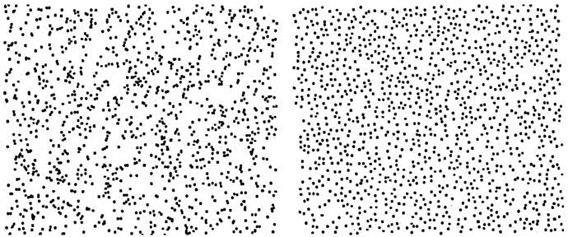
\includegraphics[scale=0.75]{images/random?} % requires the graphicx package
   \caption{Which is random?}
   \label{fig:example}
\end{figure}
The image on the left is genuine randomness, while the image on the right is too evenly spaced for it to be \emph{truly} random. In actuality, the left plots star locations while the right depicts the positions of glowworms on the ceiling of a cave in New Zealand. The glowworms spread themselves out evenly to reduce competition for food amongst themselves; the even distribution is the result of a non-random force. The right image suggests true randomness appears in clusters.

Though we will not discuss methods of generating uniform random variates, their importance to us
is not a small one. From here on we assume the existence of a random
number generator that allows us to sample $U \sim \mbox{Unif}(0,1)$. For many problems in probability, artificial intelligence, and computational statistics, exact inference is intractable and we must turn to approximations. This thesis aims to explore approximation techniques that arise from numerical sampling, or Monte Carlo methods. In a sentence, our goal will be to find the expectation of some function $h$ with respect to some probability distribution $f$. This appears in a Bayesian  setting when we would like to sample from a posterior distribution to evaluate expectations.

We begin with a simple review of random variate generation before moving to more advanced techniques that allow us to sample from more complex distributions. We begin with a
review of classical sampling (simple sampling, rejection sampling, importance sampling) before directing the majority of our attention to Monte Carlo based methods. In specific, we explore the advantages of slice sampling and gradient based Monte Carlo over traditional Markov Chain Monte Carlo simulations. In some cases we will
prove the convergence  of such Markov Chains, while in others we will point the reader in the right direction
direction. Finally, once we have covered the basics of these sampling methods, we will take a look at applications
and more recent research that allow us to speed up the traditional algorithms.
\subsection{Related works}

Many of our results are generalizations or applications of the Metropolis algorithm that first appeared in \cite{metropolis1953equation} and
was revised into the Metropolis-Hastings in \cite{hastings1970monte}. Though the naming of the actual algorithm
has been disputed (it is often asserted that Metropolis did nearly no work on the original paper and simply oversaw the co-authors), we refer to the algorithm as Metropolis-Hastings for historical reasons.  Metropolis published
his paper while working at Los Alamos Scientific Lab in the field of computational statistics. The term ``Monte Carlo"
was coined because some of the first applications were to card games, like those in the Monte Carlo Casino in Monaco. Such Monte Carlo simulations were important in the development of the Manhattan project.

Though one of the more famous samplers, the Gibbs sampler, was introduced by Stuart and Geman in 1984 \cite{geman1984stochastic} these sorts of numerical sampling techniques really became vogue again in the early 1990's arguable because of the
advent of the personal computer and wider access to more computational power. The Gibbs sampler appeared nearly two decades before Neal's slice sampler \cite{neal2003slice}, though for our purposes we will
discuss the 2D slice sampler to motivate the Gibbs sampler. We will draw heavily from \cite{mira2002efficiency}, \cite{roberts1998}, \cite{robert2004monte} in our proof of uniform ergodicity of the 2D slice sampler. Neal is also responsible for results relating to the Hybrid Monte Carlo \cite{brooks2011handbook} which uses gradient information to navigate the search space more efficiently. As a general introduction to each of these sampling
techniques, \cite{bishop2006pattern} has proven invaluable.

More recent results have been due to the proliferation of big data which, in the Bayesian setting, necessitates the ability to sample from a posterior distribution with billions of data points. Sequential hypothesis testing
has proved to reduce some of the budget required for Metropolis-Hastings \cite{korattikara2013austerity}. This technique has also been applied to the slice sampler, though the paper has not yet been published. In the later portions of this paper, we discuss these applications and their improvements on real world data.
\subsection{Prospective}
At this point I will have either given sufficient motivation for my research or will provide it here. I would like to present a few interesting (and probably difficult cases) where traditional techniques run into problems. I hope
to give a glimpse of the framework of how I think all these ideas fit together and how the reader should
conceptualize the topics presented therein.
\section{Random Variable Generation}
As stated in the introduction, we assume
we may sample $u \sim \mathcal{U}[0, 1]$. Given this, what other distributions can
we generate from? Well, we can sample from both Bernoulli and Binomial
distributions because we can generate a uniform random
variate and if $u > 0.5$ then we have ``flipped" a head. Otherwise, we have
flipped a tails.

We can take a more general approach to generating random variates
given our random number generator.

\subsection{The Inverse Transform}
\begin{defn} Suppose $X$ is a random variable
distributed according to $f_x$. We denote by $F_X$ the cumulative distribution function (cdf)
where $$F_X(x) = \pr(X \le x)$$
\end{defn}
\begin{defn} For a non-decreasing function $F$ on $\R$, the generalizes inverse of $F$, denoted
$F^{-1}$, is the function such that
$$F^{-1}(u) = \inf\{x : F(x) \le u\}$$
\end{defn}
With this in hand, we now have the tools to generate
random variates from any distribution with a computable generalized inverse.
\begin{lem} If $U \sim \mathcal{U}[0, 1]$ then $X = F^{-1}(U)$ has the distribution
$F$.
\end{lem}
\begin{proof}
\begin{align*}
\pr(X \le x) ={}& \pr(F^{-1}(U) \le x)\\
={}& \pr(U \le F(X))\\
={}& F(X)
\end{align*}
Where the second equality follows from the fact that $F$ is non-decreasing. 
\end{proof}
Thus, in order to generare a random variable $X \sim F$ we may simply
draw $U \sim \mathcal{U}[0, 1]$ and assign $X = F^{-1}(U)$. While
our initial assumption of the ability to generate uniform random variates
may have seemed trivial, we now see how important they are to our study. In fact
if the random variates we use are \emph{not} truly uniform
then the inverse transform fails to sample for the correct distribution.

To use the inverse transform we must explicitly write down
the cumulative distribution function and efficiently compute
its generalized inverse. 
\begin{exmp}
Include example/simulations for a distribution for which the inverse transform
is possible.
\end{exmp}
\begin{exmp}
The cumulative distribution function of the normal distribution
cannot be expressed in a closed for because $$\Phi(x) = \dfrac{1}{\sqrt{2\pi}}\int_{-\infty}^x e^{-z^2/2}\,dz$$
Luckily, there exist approximations of $\Phi$ and $\Phi^{-1}$ up to an arbitrary 
precision, so we may still confidently use the inverse transform to generate normal 
random variables. We are not always this lucky and must look to other methods
that allow us to sample from distributions without relying on strong analytic 
properties of our target distribution. 
\end{exmp}

\subsection{Acceptance-Rejection Sampling}
In looking for an algorithm to sample from distributions, we begin
with a theorem that we will revisit in the later section on slice sampling.
The theorem follows from the idea if $f_X$ is the density of interest, we
may write $$f_X(x) = \int_0^{f_X(x)}\,du$$
where $f_X$ appears as the marginal density of the joint distribution
$$(X, U) \sim \mathcal{U}\{(x, u) : 0 < u < f_X(x)\}$$
The introduction of the auxiliary variable $U$ allows
us to generate from our target distribution by generating uniform
random variables from the set $\{(x, u) : 0 < u < f_X(x)\}$ and then marginalizing
out $U$. We state the result more formally:
\begin{thm} 
Simulating $$X \sim f(x)$$ is equivalent to simulating $$(X, U) \sim \mathcal{U}\{(x, u)~:~0<u<f(x)\}.$$
\end{thm}
Actually sampling from the joint distribution $(X, U)$ introduces difficulty, though,
because sampling $Y \sim f_X(x)$ and $U | Y \sim \mathcal{U}[0, f_X(x)]$ defeats
the purpose of introducing the auxiliary variable. If we could sample $Y \sim f_X(x)$
we would already be done. As we will see in slice sampling, the solution
is to generate pairs $(Y, U)$ from a larger set and only accept them
if they satisfy the constraint.

We can come up with simple cases in 1-dimension if $f_X$ is bounded by $m$
and the support of $f_X$, denoted $\supp f_X$, is $(a, b)$. Sampling
pairs $(X, U) \sim \mathcal{U}[0 \le u \le m]$ is tantamount to simulating $X \sim \mathcal{U}[a, b]$
and $U|X \sim \mathcal{U}[0, m]$ and accepting the pair
only if $0 < u < f_X(x)$. This does indeed sample from
the desired distribution because
\begin{align*}
\pr(X \le x) ={}& \pr(X \le x | U \le f_X(x))\\
={}& \dfrac{\int_a^x\int_0^{f_X(x)} \frac{1}{b-a}\cdot\frac{1}{m}\,du\,dy}{\int_a^b\int_0^{f_X(x)} \frac{1}{b-a}\cdot\frac{1}{m}\,du\,dy}\\
={}&  \dfrac{\int_a^x\int_0^{f_X(x)} \,du\,dy}{\int_a^b\int_0^{f_X(x)}\,du\,dy}\\
={}&  \dfrac{\int_a^x f_X(x) \,dy}{\int_a^b f_X(x)\,dy}\\
={}& \int_a^x f_X(x) \,dy
\end{align*}
Because the denominator is the integral of a pdf over its entire support. 

This argument may be generalized to situations in which we cannot
bound either the support, $\mathcal{X}$, or mode of the distribution of interest,
so long as it remains feasible to sample uniformly over the unbounded
region. Defining the larger, or enveloping set, as
$$\mathscr{L} = \{(y, u) : 0 \le u \le Mg(y)\}$$
where $Mg(y) \ge f_Y(y)$ over the entire support. Obviously, we
could let $g$ be a uniform distribution and $M$ be a very large constant.
However, for effeciency's sake we want $Mg(y)$ to be as 
close to $f_Y(y)$ as possible; otherwise we are wasting lots of draws. Sampling
$Y \sim g$, $U |Y \sim\mathcal{U}[0, Mg(y)]$, accepting only if
$u \le f_Y(y)$ allows us to sample from $f_Y(y)$:
\begin{align*}
\pr(X \in \mathcal{A}) ={}& \pr(Y \in \mathcal{A} | U \le f_Y(y))\\
={}& \dfrac{\int_{\mathcal{A}}\int_0^{f_Y(y)} g(y) \frac{1}{Mg(y)} \, du\,dy}{
\int_{\mathcal{Y}}\int_0^{f_Y(y)} g(y) \frac{1}{cg(y)} \, du\,dy
}\\
={}& \dfrac{\int_{\mathcal{A}}f_Y(y)\,dy}{\int_{\mathcal{Y}}f_Y(y)\,dy}\\
={}& \int_{\mathcal{A}}f_Y(y)\,dy
\end{align*}
A similar computation shows that
\begin{align*}
\pr(\mbox{accept}) = {}& \int_{\mathcal{A}}\int_0^{f_Y(y)} g(y) \frac{1}{Mg(y)} \, du\,dy\\
={}& \dfrac{1}{m} \int_{\mathcal{A}}f_Y(y)\,dy
\end{align*}
So that the fraction of points rejected depends on our constant $M$; the larger
$M$ is, the more points we must reject.

This result leads to a generalization of the fundamental theorem of
simulation.
\begin{thm}
Let $X \sim f_X(x)$ and let $g(x)$ be a density function that satisfies
$f_X(x) \le Mg(x)$ for some $M \ge 1$. Then, to simulate $X \sim f$, it
is sufficient to simulate
$$Y \sim g\hspace{15pt}\mbox{and}\hspace{15pt} U | Y \sim \mathcal{U}[0, Mg(y)]$$
and accept if $u \le f_X(x)$
\end{thm}
This leads directly to the Accept-Reject algorithm, which is an implementation
of this theorem.
\begin{algorithm}
\caption{Accept-Reject Sample}
\begin{algorithmic}[1]
\Procedure{}{}
\State Generate $X \sim g$, $U \sim \mathcal{U}[0, Mg(X)]$
\State Accept $Y = X$ if $U \le f_Y(X)$
\State Return to 1 otherwise.
\EndProcedure
\end{algorithmic}
\end{algorithm}
\subsection{Adaptive Rejection Sampling}

\section{Monte Carlo Methods}

\begin{defn}
A sequence of random variables 
$X_1, \ldots, X_n$ is a Markov chain if
\begin{equation}
\pr(X_{n + 1} | X_n, X_{n-1}, \ldots, X_1) =\pr(X_{n + 1} | X_n) 
\end{equation}
\end{defn}
The defining characteristic of a Markov chain is that the conditional
distribution of $X_{n+1}$ is solely dependent on $X_n$. We define our state
space as the set of values $X_i$ may take. Every Markov chain has an initial
distribution, $\mu$, where $\pr{(X_1 = x_i)}$ and a transition function $P$. If the state
space is finite and $X$ may take on values in the range $\{x_1, \ldots, x_n\}$ 
then we define the transition function $P$ as $$P(i, j) = \pr{(X_{n+1} = x_j | X_{n} = x_i)} = p_{ij}$$
For our purposes, we deal mostly with uncountably infinite state spaces in which we
consider the initial distribution as an unconditional probability distribution
and the transition function as a conditional probability distribution. Note that
stationarity implies that $P$ is invariant, or that it's values remain stationary.
However, the reverse is not necessarily true.

Given a transition function and an initial distribution $\mu_0$, the marginal
probability of the $X_1$ is obtained by matrix multiplication $$\mu_1 = \mu P$$
and similarly, $X_n \sim \mu_n = \mu P^n$. Thus, we see that once the initial
state is given, the entire chain is dependent on $P$.

We now take a moment to discuss the properties of Markov chains that will 
be necessary for us to prove convergence of certain sampling routines.
\subsection{Properties of Markov Chains}
\subsubsection{Stationarity}
A stochastic process is stationary if for every positive integer $k$
the distribution of the $k$-tuple
$$(X_{n+1}, \ldots, X_{n+k})$$ does not depend on $n$. Similarly, 
the probability of $(X_{n+2}, \ldots, X_{n+k})$ given $X_{n+1}$ does
not depend on $n$. We call a Markov Chain Stationary iff the marginal distribution of $X_n$
does not depend on $n$.



Markov Chain Monte Carlo simulations use Markov chains whose stationary distribution, $\pi$, we wish to sample from. By initializing the Markov chain with an initial state and transition probabilities, we may run the chain for a ``sufficient" number of steps to draw samples from the desired distribution. It is common to ignore some number of samples at the beginning (burn-in), and then consider only every $n^{{th}}$ sample when computing an expectation.

\subsubsection{Irreducibility}
Irreducibility is another important property of Markov chains which says that
regardless of the current state of the chain, it is possible to reach any other
state in a finite amount of time.
\begin{defn}
A Markov chain is \emph{irreducible} if $\exists
m < \infty$ such that
$$\pr{(X_{n+m} = x_j | X_n = x_i)} \ge 0$$
for all $i, j$. 
\end{defn}
The property of irreducibility is a first measure of the sensitivity of the Markov chain
to the initial conditions (Casella, Springer). Once we have shown the irreducibility
of a chain, it guarantees convergence.

\begin{defn}
A set $C$ is \emph{small} if there exists an $m > 0$ and a nonzero measure
$\nu_m$ such that $$P^m(x, x') \ge\nu_m(x_{m})$$
for all $x \in C$ and for all $x' \in \mathcal{B}(\mathcal{X})$
\end{defn}
We may also call a set $C$ small if there exists a constant $\epsilon > 0$ and a probability measure 
$\nu$ such that $$P(x, A) \ge \epsilon\nu(A), \hspace{10pt} \forall x\in C, \forall A \in \mathcal{B}(\mathcal{X})$$
What's the intuition behind this?
\subsubsection{Aperiodicity}
The period of a state in a Markov chain tells us
how often we will visit that state. An aperiodic
chain is one in which 

\subsubsection{Ergodicity}
\begin{defn} The Markov chain $(X_n)$ is \emph{uniformy ergodic} if 
$$\lim_{n\to\infty}\sup_{x\in\mathcal{X}} \|P^n(x, \cdot) - \pi \|_{TV} = 0$$
\end{defn}
In attempting to show uniform ergodicity, we will make use of the following theorem.
\begin{thm}
The following are equivalent:
\begin{enumerate}[(a)]
\item $(X_n)$ is uniformly ergodic;
\item there exist $R \le \infty$ and $r$ such that
$$\|P^n(x, \cdot) - \pi \|_{TV} < Rr^{-n}, \hspace{10pt} \forall x\in\mathcal{X};$$
\item $(X_n)$ is aperiodic and $\mathcal{X}$ is a small set;
\item $(X_n)$ is aperiodic and there exist a small set C and a real $\kappa > 1$
such that
$$\sup_{x\in\mathcal{X}} \mathbb{E}_x[k^{\tau C}] <\infty$$
\end{enumerate}
\end{thm}
If the whole space $\mathcal{X}$ is small, there exist a probability distribution,
$\phi$, on $\mathcal{X}$, constants $\epsilon < 1$ and $\delta > 0$,
and $n$ such that, if $\phi(A) > \epsilon$ then
$$\inf_{x\in\mathcal{X}} P^n(x, A) > \delta$$
We see here the relation between analytical limits and uniform ergodicity,
giving us an intuition behind the strength of uniform ergodicity. In later chapters,
this property is refered to as \emph{Doeblin's condition}.

\subsection{Markov Chain Monte Carlo}
Although the sampling techniques we have discussed worked well, they required us to 
have a closed form cdf of the target distribution. As we will see, the previous approaches also fail as we move to higher dimensional space and the curse of dimensionality sets in. We turn to Markov Chain Monte Carlo simulations because they ameliorate many of the problems faced by classical sampling.


A Monte Carlo simulation allows us to approximate the probability of certain outcomes by running a large number of
trials to obtain an empirical distribution of possible events. 
Markov Chain Monte Carlo simulations use Markov chains whose stationary (equilibrium) distribution we wish to sample from. By initializing the Markov chain with an initial state and transition probabilities, we may run the chain for a ``sufficient" number of steps to draw samples from the desired distribution. It is common to ignore some number of samples at the beginning (burn-in), and then consider only every $n^{{th}}$ sample when computing an expectation.

\subsection{Metropolis Hastings}
This section will provide an in-depth look at the Metropolis-Hastings
algorithm. It is here that we will really begin to build our understanding of
how Markov Chain Monte Carlo methods operate concretely. It is here that we
will also be able to take a look at the different convergence properties of 
MCMC algorithms. We will begin with a few instances where Metropolis-Hastings does
well but eventually we will move to cases in which the approach fails, indicating that
there are better ways to be doing this.

\section{Slice Sampling}
As before, we desire to sample from a distribution, $f(x)$, that we know
up to a normalizing factor (i.e. $f(x) = f_1(x)/Z_p$) and may easily evaluate.
We turn now to a technique that is more robust to hyperparameter tuning, such
as the step size in Metropolis-Hastings.

Slice sampling draws samples from the volume 
under the curve of $f_1(x)$. If we imagine our target
distribution on a dart board which we throw a million darts at,
slice sampling removes all the darts above the curve of the distribution
so that we are left with the desired pdf.
More specifically, in one dimension, slice sampling provides a method for making transitions
from a two-dimensional point $(x, u)$ lying under 
the curve $f_1(x)$ another point $(x', u')$ lying under the same curve,
such that the probability distribution of $(x, u)$ tends to a uniform distribution
over the area under the curve $f_1(x)$ (Mackay, Chapter 29, 
http://www.cs.toronto.edu/~mackay/itprnn/ps/358.386.pdf).
\begin{algorithm}
\caption{A Slice Sample}\label{euclid}
\begin{algorithmic}[1]
\Procedure{}{}
\State Evaluate $f_1(x_{t})$
\State Draw a vertical coordinate $u_{t+1} \sim Uniform[0, f_1(x_{t})]$
\State Create a horizontal interval $(x_l, x_r)$ enclosing $x_{t}$
\BState \emph{loop}:
\State Draw $x_{t+1} \sim Uniform(x_l, x_r)$
\If {$f_1(x_{t+1}) > u_{t+1}$} \Return $x_{t+1}$
\Else~Modify the interval $(x_l, x_r)$ and \textbf{goto} \emph{loop}
\EndIf
\EndProcedure
\end{algorithmic}
\end{algorithm}


Although both slice samplers and Metropolis samplers
navigate the sample space by random walk, the slice sampler
is able to adaptively update its step size to match the characteristics
of the distribution whereas a Metropolis
sampler must have this value chosen a priori. A disadvantage of the Metropolis-Hastings
algorithm is its dependence on a good proposal
distribution. A slice sampler is able to adjust its window in linear time, 
whereas a traditional Metropolis
sampler does this in quadratic time. Moreover, there are no rejections
in slice sampling.

As we will see later in the Hybrid Monte Carlo, slice sampling introduces
an auxiliary variable $f_1\hat{p}$. We eventually marginalize out the
auxiliary variable to sample from the desired distribution. The key insight of slice sampling
is that drawing a sample from the distribution of $f_1(x)$ is the same
as uniformly sampling from the points underneath the curve of such a distribution,
as we saw the the darts example. 
Concretely, we want all the points $(x, u)$ such that $0 \le u \le f_1(x)$ 
where $\dfrac{f_1(x)}{Z_p} = f(x)$ and $Z_p = \int f_1(x)\,dx$. 

To achieve this, note that $Z_p$ is literally the area under the curve
of $f_1(x)$ so that uniformly choosing a single point $(x, u)$ occurs
with probability $1/Z_p$. Thus, samples are then drawn from the joint distribution
$f(x, u)$ given by
 \begin{displaymath}
   f(x, u) = \left\{
     \begin{array}{lr}
        \dfrac{1}{Z_p} &\mbox{if}~0 \le u \le f_1(x)\\
       0 & \text{otherwise}
     \end{array}
   \right.
\end{displaymath} 
So that the marginal distribution of $x$ is given by
$$\int f(x, u) du = \int_0^{f_1(x)}\dfrac{1}{Z_p}du =\dfrac{f_1(x)}{Z_p} = f(x)$$
To sample from $f(x, u)$ we employ Gibbs sampling in which we alternate
sampling $x$ and $u$. 


To see that the successive sampling preserves the uniform distribution on the subgraph of 
$f_1(x)$, note that if $x_{t} \sim f(x)$ and $u_{t+1} \sim
\mathcal{U}[0, f_1(x_{t})]$ then $$(x_{t}, u_{t+1}) \sim f(x_{t})\dfrac{\mathbb{I}(0 \le u_{t+1} \le f_1(x_{t})}{f_1(x_{t})} \propto \mathbb{I}(0 \le u_{t+1} \le f_1(x_{t})$$
And if $x_{t+1} \sim \mathcal{U}[A_{t+1}]$ where $A_{t+1} = \{x : ~f(x) \ge u_{t+1}\}$ then $$(x_{t}, u_{t+1}, x_{t+1}) \sim f(x_{t})\dfrac{\mathbb{I}(0 \le u_{t+1} \le f_1(x_{t})}{f_1(x_{t})}\dfrac{\mathbb{I}(x_{t+1} \in A_{t+1})}{\mu(A_{t+1})}$$
Where $\mu(A_{t+1})$ denotes the measure of the set. Thus
\begin{align*}
(u_{t+1}, x_{t+1}) \sim{}& C \int \mathbb{I}_{0\le u \le f_1(x)}\dfrac{\mathbb{I}_{u \le f_1(x_{t+1})}}{\mu(A_{t+1})}\,dx\\
={}& C\mathbb{I}_{0\le u \le f_1(x_{t+1})} \int \dfrac{\mathbb{I}_{u \le f_1(x)}}{\mu(A_{t+1})}\,dx\\
\propto{}& \mathbb{I}_{0\le u \le f_1(x_{t+1})}
\end{align*}

\subsection{Uniform Ergodicity of the Slice Sampler}
For the simple case of the $2D$ slice sampler, if we denote
by $\mu(\omega)$ the Lebesgue measure of the set
$$\mathcal{L}(\omega) = \{y : f_i(y) \ge \omega\}$$
the cdf of the transition kernel gives
\begin{align*}
\pr\bigg(f_1(X_{t+1} \le \eta)~|~f_x(X_t) = v\bigg) ={}& \int\int \dfrac{\mathbb{I}(0 \le \omega \le v)}{v}\cdot
\dfrac{\mathbb{I}(\omega \le f_1(x) \le v)}{\mu(\omega)}\,d\omega dx
\end{align*}
Where we first draw $\omega$ uniformly on $[0, v]$ and then draw $X_{t+1}$
uniformly on $\mathcal{L}(\omega)$. Continuing gives
\begin{align*}
\pr\bigg(f_1(X_{t+1} \le \eta)~|~f_x(X_t) = v\bigg) ={}& \dfrac{1}{v}\int\dfrac{\mathbb{I}(0 \le \omega \le v)}{\mu(\omega)}\int \mathbb{I}(\omega \le f_1(x) \le v)\,d\omega dx\\
={}& \dfrac{1}{v}\int
\dfrac{\mu(\omega) - \mu(\eta)}{\mu(\omega)}\cdot\mathbb{I}(0 \le \omega \le v)\,d\omega\\
={}&\dfrac{1}{v}\int_0^{\min(\eta, v)}
\dfrac{\mu(\omega) - \mu(\eta)}{\mu(\omega)}\,d\omega\\
={}&\dfrac{1}{v}\int_0^v
\max\bigg(1 -\dfrac{\mu(\eta)}{\mu(\omega)}, 0\bigg)\,d\omega
\end{align*}
Which shows that the convergence properties are total dependent on the measure, $\mu$.
Now, for the main result which we owe Tierney and Mira (1999) who, under
boundess conditions, established the following result.
\begin{lem}
If $f_1$ is bounded and $\mbox{supp}~f_1$ is bounded, the 2D slice sampler
is uniformly ergodic.
\end{lem}
\begin{proof}
Without loss of generality, assume that $f_1$ is bounded by 1 and that 
$\mbox{supp}~f_1$ is equal to $(0, 1)$. To prove uniform ergodicity, 
we will show that the $\mbox{supp}~f_1$ is a small set so that we may invoke
Doeblin's condition.
Let $$\xi(v) = \pr\bigg(f_1(X_{t+1} \le \eta)~|~f_x(X_t) = v\bigg)$$
Note that when $\omega > \nu$, i.e. when $\mu(\nu) > \mu(\omega)$ this probability is 0.
However, when $v \ge \eta$,
$$\xi(v) = \dfrac{1}{v}\int_0^\eta
1 -\dfrac{\mu(\eta)}{\mu(\omega)}\,d\omega$$
is decreasing in $v$ since it only appears in the denominator outside of the integral.
When $v \le \eta$ we recognize $$\xi(v) = \dfrac{1}{v}\int_0^v
1 -\dfrac{\mu(\eta)}{\mu(\omega)}\,d\omega$$ as the average of the
function $1 -\dfrac{\mu(\eta)}{\mu(\omega)}$
where $\omega$ is uniformly distributed on $[0, v]$. The larger $\omega$,
the smaller the measure of $\mathcal{L}(\omega)$ is because there is less of 
$f_1$ above it. We conclude that $\mu(\omega)$ is decreasing in $\omega$ and thus also decreasing in $v$. 
Hence, $\xi(v)$ is decreasing in $v$ for all $\eta$. If we think about this more,
it would not make sense if it were increasing because that would imply that
we wouldn't be spending enough time in the modes; i.e. the larger $v$ 
the more likely we are to end up \emph{below} some threshold (away from the mode).
To find bounds on the cdf of the transition kernal we first find the minimum
\begin{align*}
\lim_{v \to 1}\xi(v) ={}&\int_0^\eta 1 - \dfrac{\mu(\eta)}{\mu(\omega)}\,d\omega
\end{align*}
which is bounded above by $\int_0^\eta 1 \,d\omega = \mu(\eta)$ and below by $0$. 
The maximum then is
\begin{align*}
\lim_{v \to 0}\xi(v) ={}&\lim_{v \to 0}\dfrac{\int_0^v 1 - \dfrac{\mu(\eta)}{\mu(\omega)}\,d\omega}{v}\\
={}& \lim_{v \to 0} 1 - \dfrac{\mu(\eta)}{\mu(v)}\\
={}& 1 - \mu(\eta)
\end{align*}
by L'Hopital's rule which is bounded above by 1 and below by 0. By finding
nondegenerate upper and lower bounds on the cdf of the transition kernel, we may
derive Doeblin's condition and thus uniform ergodicity. The entire support
of $f_1$ is thus a small set and uniform ergodicity follows (does it? what about aperiodicity?).
\end{proof}

Our implementation of the slice sampler may be seen below
\begin{Schunk}
\begin{Sinput}
> dist.x <- seq(-10, 10, length = 1000)
> Slice.Sample <- function(x0, f, nsample, step = 1) {
+   x <- c(x0)
+   for (i in 2:nsample) {
+     u <- runif(1, 0, f(x[i - 1]))
+     l <- x[i - 1] - 1
+     r <- x[i - 1] + 1
+     while (u < f(l)) {
+       l <- l - step
+     }
+     while (u < f(r)) {
+       r <- r + step
+     }
+     while (TRUE) {
+       x.proposal <- runif(1, l, r)
+       if (u < f(x.proposal)) {
+         x[i] <- x.proposal
+         break
+       } else { # drew sample above curve, must shrink slice
+         if (x.proposal < l) {
+           l <- x.proposal
+         } else if (x.proposal > r) {
+           r <- x.proposal
+         }
+       }
+     }
+   }
+   return(x)
+ }
> density <- function(x) { 
+   return(dnorm(x, -2, 0.4) + 3 * dnorm(x, 1, 0.5) + dnorm(x, 4, 0.4))
+ }
> hist(Slice.Sample(1, density, 1000, 1), breaks = 100, prob = T)
\end{Sinput}
\end{Schunk}
\includegraphics{thesis_draft_2-001}

\subsection{Reflective Slice Sampling}
Here we assume that we are able to compute both $\hat{p}(x)$ and its gradient. We proceed 
as before and draw uniformly from $[0, \hat{p}(x)]$ to define a $n$-dimensional
slice. We also introduce $n$ momentum variables, written as a vector $\vec{r}$
which indicate the current direction and speed of motion through state space.
At each iteration, we sample $\vec{r}$ and repeatedly update $x$ by stepping
in the direction of $r$ for some number of steps before arriving at
our new proposal.

We use the gradient to tell us how we should update the momentum when we
are pushed out of the target distribution. The reflected momentum direction is 
a function of the incident momentum and the partial derivatives.

\subsection{Refractive Slice Sampling}
Here and in the following section we touch on variations of the slice sampler.
At this point it is not clear to what extent we will deal with them. It may
very well be the case that we explain what they are and how the sample without delving into
the finer details such as convergence as we did with the standard slice sampler.
\subsection{Elliptical Slice Sampling}

\section{Gibbs Sampling}
The slice sampler leads fairly nicely into Gibbs sampling because
the successive steps in slice sampling are actually
Gibbs sampling steps. 
Below is an implementation of such a Markov Chain Monte Carlo sampler, a Gibbs 
Sampler which will sample from a 2D exponential.
\begin{Schunk}
\begin{Sinput}
> Exp.Bounded <- function(rate, B) {
+   # rexpT samples from the exponential distribution
+   # until a value less than B is observed
+   x <- rexp(1, rate)
+   while (x > B) {
+     x <- rexp(1, rate)
+   }
+   return(x)
+ }
> Gibbs.Sampler <- function(M, B) {
+   # Gibbs.Sampler uses the Gibbs sampling method
+   # to sample from a joint distribution given our
+   # knowledge of the condition distributions.
+   mat <- matrix(ncol=2, nrow = M)
+   x <- 1
+   y <- 1
+   mat[1, ] <- c(x, y)
+   for (i in 2:M) {
+       x <- Exp.Bounded(y, B)
+       y <- Exp.Bounded(x, B)
+       mat[i,] <- c(x, y)
+   }
+   layout(matrix(c(1,1,2,3), 2, 2, byrow = TRUE))
+   plot(mat, main="Joint Distribution", xlab="X",ylab="Y")
+   hist(mat[ , 1], main="Marginal dist. of X", xlab="X")
+   hist(mat[ , 2], main="Marginal dist. of Y", xlab="Y")
+ }
\end{Sinput}
\end{Schunk}
\begin{Schunk}
\begin{Sinput}
> Gibbs.Sampler(1000, 10)
\end{Sinput}
\end{Schunk}
\includegraphics{thesis_draft_2-gibbsSampler}

\section{Hamiltonian Monte Carlo}
The Hamiltonian Monte Carlo, along with slice sampling, will be one of the ``set
pieces" of this paper. That is, it will be one of the more in-depth sections.
\subsection{Hamiltonian Physics}
Here we give an introduction to Hamiltonian physics and give an example
of a simple system we can model with it (for instance a puck sliding over a
raised, friction less surface). We will also discuss the physical interpretation. 
A canonical ensemble is the statistical ensemble used to represent the possible
states of a mechanical system in thermal equilibrium with a heat bath. The 
idea that ``a statistical ensemble is a probability distribution for the state 
of the system." was introduced by J. Willard Gibbs in 1902 (Elementary Principles in Statistical Mechanics).
\subsection{Symplectic Geometry}
Certain properties of symplectic geometry allow us to make the analogy between
Hamiltonian physics and Markov Chain Monte Carlo. We discuss those 
important details in this section to elucidate some of the deeper aspects
of the physical interpretation of Hamiltonian systems.
\section{Improvements}
\subsection{Results}
I would like to end by giving a comparison of the many techniques we discussed
over the course of the paper. In their respective sections, we have have used
toy examples to demonstrate how a sampler worked. Here, I would like to present
the samplers with degenerate distributions and see how they perform. 
\subsection{Moving forward}
Given the shortcoming we find in the previous section, we will cover the ways
in which we may attempt to ameliorate them. This may involve
novel research or it may involve introducing variant of certain samplers,
as we did with the slice sampler
\section{Conclusion}
I think this is pretty self-explanatory. We will tie up any loose ends, though 
most of them will have been taken care of in the previous section.
\bibliographystyle{plain}
\bibliography{thesis_bibliography}{}
\end{document}
